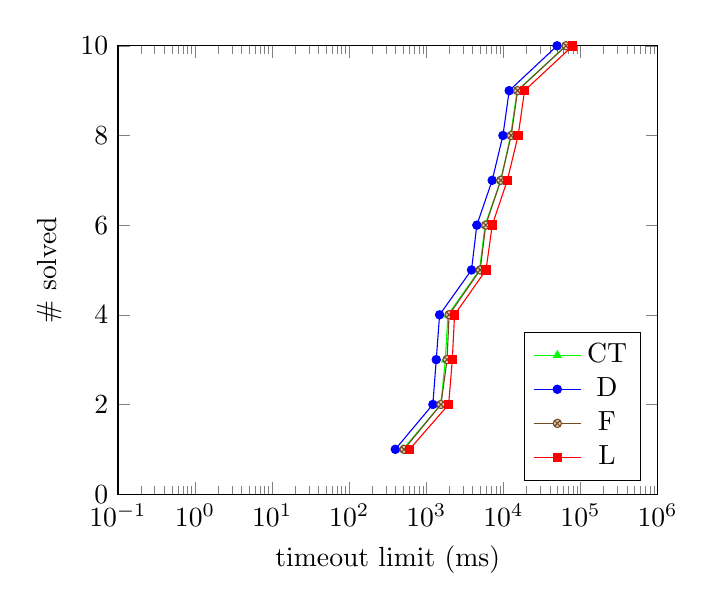
\begin{tikzpicture}[scale=1.0]
  \begin{axis}[
    xmode=log,
    ymin=0,ymax=10,
    xmin=0.1, xmax=1000000,
    every axis plot/.style={thin},
    xlabel={timeout limit (ms)},
    ylabel={\# solved},
    legend pos=south east
    % table/create on use/cumulative distribution/.style={
    %   create col/expr={\pgfmathaccuma + \thisrow{f(x)}}   
    % }
    ]
    \addplot 
    [mark=triangle*,
    mark size=1.5,
    mark options={solid},
    green] 
    coordinates {(497.040, 1)
(1547.756, 2)
(1763.726, 3)
(1907.137, 4)
(4902.199, 5)
(5780.408, 6)
(9243.288, 7)
(12406.243, 8)
(15073.489, 9)
(64243.147, 10)};

    \addplot 
    [blue,
    mark=*,
    mark size=1.5,
    mark options={solid}]
    coordinates {(395.959, 1)
(1215.821, 2)
(1345.530, 3)
(1486.577, 4)
(3857.618, 5)
(4519.651, 6)
(7153.142, 7)
(9856.387, 8)
(11891.137, 9)
(49653.082, 10)};

    \addplot [brown!60!black,
    mark options={fill=brown!40},
    mark=otimes*,
    mark size=1.5]
    coordinates {(514.223, 1)
(1547.139, 2)
(1859.368, 3)
(1973.813, 4)
(4998.683, 5)
(5897.494, 6)
(9245.556, 7)
(12617.058, 8)
(15292.670, 9)
(64928.990, 10)};

    \addplot 
    [red,
    mark size=1.5,
    mark=square*]
    coordinates {(606.873, 1)
(1947.577, 2)
(2174.187, 3)
(2324.305, 4)
(5946.616, 5)
(7162.402, 6)
(11233.842, 7)
(15540.199, 8)
(18806.011, 9)
(79114.731, 10)};
    \legend{CT,D,F,L}
  \end{axis}
\end{tikzpicture}
